\documentclass[border=6pt]{standalone}
\usepackage{newtxtext}\usepackage{xcolor}\usepackage{tikz}
\definecolor{tier0}{HTML}{86B6EF}\definecolor{tier1}{HTML}{5598E7}\definecolor{tier2}{HTML}{2A78D6}
\definecolor{tier3}{HTML}{1C5CAB}\definecolor{tier4}{HTML}{104281}
\definecolor{gridcol}{HTML}{E4E3DF}\definecolor{inkmuted}{HTML}{5F5E5A}
\definecolor{orangeborder}{RGB}{181,133,84}\definecolor{orangefill}{RGB}{245,229,210}
\definecolor{blueborder}{RGB}{72,98,220}\definecolor{bluefill}{RGB}{227,237,248}
\definecolor{greenborder}{RGB}{74,166,74}\definecolor{greenfill}{RGB}{226,241,226}
\definecolor{purpleborder}{RGB}{132,94,194}\definecolor{purplefill}{RGB}{236,230,247}
\definecolor{tealborder}{RGB}{43,140,140}\definecolor{tealfill}{RGB}{223,242,242}
\begin{document}
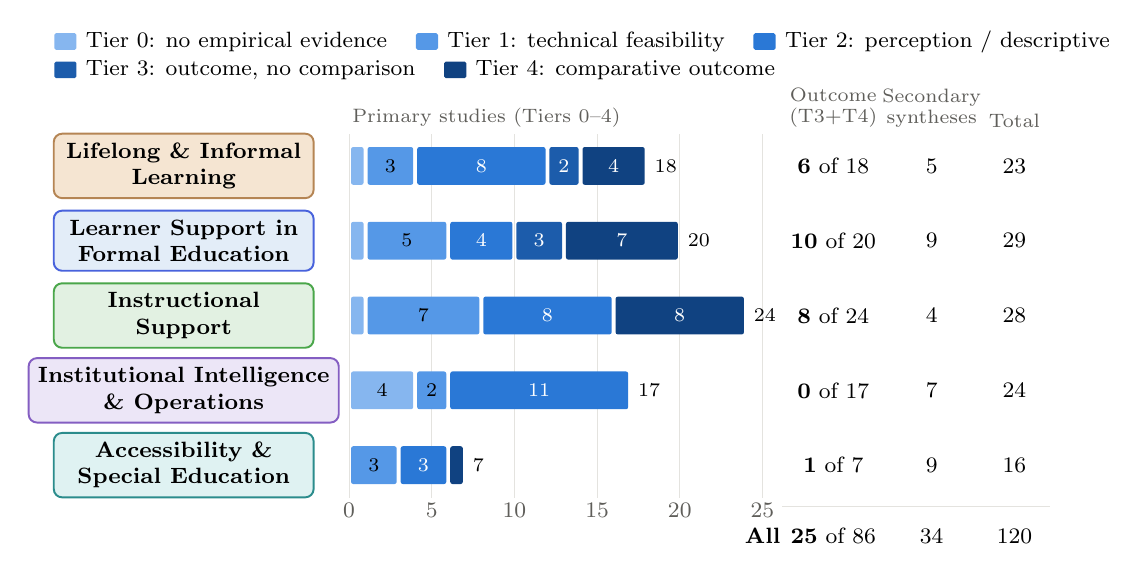
\begin{tikzpicture}[x=1cm,y=1cm,font=\footnotesize]
\node[anchor=west, inner sep=0pt, minimum width=8pt, minimum height=6pt, fill=tier0, rounded corners=0.6pt] (sw0) at (0,0.98) {};
\node[anchor=west, inner sep=1pt] (lg0) at ([xshift=2pt]sw0.east) {\footnotesize Tier 0: no empirical evidence};
\node[anchor=west, inner sep=0pt, minimum width=8pt, minimum height=6pt, fill=tier1, rounded corners=0.6pt] (sw1) at ([xshift=9pt]lg0.east) {};
\node[anchor=west, inner sep=1pt] (lg1) at ([xshift=2pt]sw1.east) {\footnotesize Tier 1: technical feasibility};
\node[anchor=west, inner sep=0pt, minimum width=8pt, minimum height=6pt, fill=tier2, rounded corners=0.6pt] (sw2) at ([xshift=9pt]lg1.east) {};
\node[anchor=west, inner sep=1pt] (lg2) at ([xshift=2pt]sw2.east) {\footnotesize Tier 2: perception / descriptive};
\node[anchor=west, inner sep=0pt, minimum width=8pt, minimum height=6pt, fill=tier3, rounded corners=0.6pt] (sw3) at (0,0.62) {};
\node[anchor=west, inner sep=1pt] (lg3) at ([xshift=2pt]sw3.east) {\footnotesize Tier 3: outcome, no comparison};
\node[anchor=west, inner sep=0pt, minimum width=8pt, minimum height=6pt, fill=tier4, rounded corners=0.6pt] (sw4) at ([xshift=9pt]lg3.east) {};
\node[anchor=west, inner sep=1pt] (lg4) at ([xshift=2pt]sw4.east) {\footnotesize Tier 4: comparative outcome};
\node[anchor=south west, inner sep=1pt, text=inkmuted] at (3.75,-0.15) {\scriptsize Primary studies (Tiers 0--4)};
\node[anchor=south, inner sep=1pt, text=inkmuted, align=center] at (9.90,-0.15) {\scriptsize Outcome\\[-2pt]\scriptsize (T3+T4)};
\node[anchor=south, inner sep=1pt, text=inkmuted, align=center] at (11.15,-0.15) {\scriptsize Secondary\\[-2pt]\scriptsize syntheses};
\node[anchor=south, inner sep=1pt, text=inkmuted] at (12.20,-0.15) {\scriptsize Total};
\draw[gridcol, line width=0.3pt] (3.75,-0.20) -- (3.75,-4.82);
\node[anchor=north, text=inkmuted, inner sep=1.5pt] at (3.75,-4.82) {\footnotesize 0};
\draw[gridcol, line width=0.3pt] (4.80,-0.20) -- (4.80,-4.82);
\node[anchor=north, text=inkmuted, inner sep=1.5pt] at (4.80,-4.82) {\footnotesize 5};
\draw[gridcol, line width=0.3pt] (5.85,-0.20) -- (5.85,-4.82);
\node[anchor=north, text=inkmuted, inner sep=1.5pt] at (5.85,-4.82) {\footnotesize 10};
\draw[gridcol, line width=0.3pt] (6.90,-0.20) -- (6.90,-4.82);
\node[anchor=north, text=inkmuted, inner sep=1.5pt] at (6.90,-4.82) {\footnotesize 15};
\draw[gridcol, line width=0.3pt] (7.95,-0.20) -- (7.95,-4.82);
\node[anchor=north, text=inkmuted, inner sep=1.5pt] at (7.95,-4.82) {\footnotesize 20};
\draw[gridcol, line width=0.3pt] (9.00,-0.20) -- (9.00,-4.82);
\node[anchor=north, text=inkmuted, inner sep=1.5pt] at (9.00,-4.82) {\footnotesize 25};
\node[draw=orangeborder, fill=orangefill, line width=0.7pt, rounded corners=3pt, minimum width=3.3cm, minimum height=0.72cm, align=center, font=\footnotesize\bfseries] at (1.65,-0.60) {Lifelong \& Informal\\Learning};
\fill[tier0, rounded corners=0.8pt] (3.775,-0.84) rectangle (3.935,-0.36);
\fill[tier1, rounded corners=0.8pt] (3.985,-0.84) rectangle (4.565,-0.36);
\node[text=black, inner sep=0pt] at (4.275,-0.60) {\scriptsize 3};
\fill[tier2, rounded corners=0.8pt] (4.615,-0.84) rectangle (6.245,-0.36);
\node[text=white, inner sep=0pt] at (5.430,-0.60) {\scriptsize 8};
\fill[tier3, rounded corners=0.8pt] (6.295,-0.84) rectangle (6.665,-0.36);
\node[text=white, inner sep=0pt] at (6.480,-0.60) {\scriptsize 2};
\fill[tier4, rounded corners=0.8pt] (6.715,-0.84) rectangle (7.505,-0.36);
\node[text=white, inner sep=0pt] at (7.110,-0.60) {\scriptsize 4};
\node[anchor=west, inner sep=1pt] at (7.59,-0.60) {\scriptsize 18};
\node[inner sep=1pt] at (9.90,-0.60) {\footnotesize\textbf{6} of 18};
\node[inner sep=1pt] at (11.15,-0.60) {\footnotesize 5};
\node[inner sep=1pt] at (12.20,-0.60) {\footnotesize 23};
\node[draw=blueborder, fill=bluefill, line width=0.7pt, rounded corners=3pt, minimum width=3.3cm, minimum height=0.72cm, align=center, font=\footnotesize\bfseries] at (1.65,-1.55) {Learner Support in\\Formal Education};
\fill[tier0, rounded corners=0.8pt] (3.775,-1.79) rectangle (3.935,-1.31);
\fill[tier1, rounded corners=0.8pt] (3.985,-1.79) rectangle (4.985,-1.31);
\node[text=black, inner sep=0pt] at (4.485,-1.55) {\scriptsize 5};
\fill[tier2, rounded corners=0.8pt] (5.035,-1.79) rectangle (5.825,-1.31);
\node[text=white, inner sep=0pt] at (5.430,-1.55) {\scriptsize 4};
\fill[tier3, rounded corners=0.8pt] (5.875,-1.79) rectangle (6.455,-1.31);
\node[text=white, inner sep=0pt] at (6.165,-1.55) {\scriptsize 3};
\fill[tier4, rounded corners=0.8pt] (6.505,-1.79) rectangle (7.925,-1.31);
\node[text=white, inner sep=0pt] at (7.215,-1.55) {\scriptsize 7};
\node[anchor=west, inner sep=1pt] at (8.01,-1.55) {\scriptsize 20};
\node[inner sep=1pt] at (9.90,-1.55) {\footnotesize\textbf{10} of 20};
\node[inner sep=1pt] at (11.15,-1.55) {\footnotesize 9};
\node[inner sep=1pt] at (12.20,-1.55) {\footnotesize 29};
\node[draw=greenborder, fill=greenfill, line width=0.7pt, rounded corners=3pt, minimum width=3.3cm, minimum height=0.72cm, align=center, font=\footnotesize\bfseries] at (1.65,-2.50) {Instructional\\Support};
\fill[tier0, rounded corners=0.8pt] (3.775,-2.74) rectangle (3.935,-2.26);
\fill[tier1, rounded corners=0.8pt] (3.985,-2.74) rectangle (5.405,-2.26);
\node[text=black, inner sep=0pt] at (4.695,-2.50) {\scriptsize 7};
\fill[tier2, rounded corners=0.8pt] (5.455,-2.74) rectangle (7.085,-2.26);
\node[text=white, inner sep=0pt] at (6.270,-2.50) {\scriptsize 8};
\fill[tier4, rounded corners=0.8pt] (7.135,-2.74) rectangle (8.765,-2.26);
\node[text=white, inner sep=0pt] at (7.950,-2.50) {\scriptsize 8};
\node[anchor=west, inner sep=1pt] at (8.85,-2.50) {\scriptsize 24};
\node[inner sep=1pt] at (9.90,-2.50) {\footnotesize\textbf{8} of 24};
\node[inner sep=1pt] at (11.15,-2.50) {\footnotesize 4};
\node[inner sep=1pt] at (12.20,-2.50) {\footnotesize 28};
\node[draw=purpleborder, fill=purplefill, line width=0.7pt, rounded corners=3pt, minimum width=3.3cm, minimum height=0.72cm, align=center, font=\footnotesize\bfseries] at (1.65,-3.45) {Institutional Intelligence\\\& Operations};
\fill[tier0, rounded corners=0.8pt] (3.775,-3.69) rectangle (4.565,-3.21);
\node[text=black, inner sep=0pt] at (4.170,-3.45) {\scriptsize 4};
\fill[tier1, rounded corners=0.8pt] (4.615,-3.69) rectangle (4.985,-3.21);
\node[text=black, inner sep=0pt] at (4.800,-3.45) {\scriptsize 2};
\fill[tier2, rounded corners=0.8pt] (5.035,-3.69) rectangle (7.295,-3.21);
\node[text=white, inner sep=0pt] at (6.165,-3.45) {\scriptsize 11};
\node[anchor=west, inner sep=1pt] at (7.38,-3.45) {\scriptsize 17};
\node[inner sep=1pt] at (9.90,-3.45) {\footnotesize\textbf{0} of 17};
\node[inner sep=1pt] at (11.15,-3.45) {\footnotesize 7};
\node[inner sep=1pt] at (12.20,-3.45) {\footnotesize 24};
\node[draw=tealborder, fill=tealfill, line width=0.7pt, rounded corners=3pt, minimum width=3.3cm, minimum height=0.72cm, align=center, font=\footnotesize\bfseries] at (1.65,-4.40) {Accessibility \&\\Special Education};
\fill[tier1, rounded corners=0.8pt] (3.775,-4.64) rectangle (4.355,-4.16);
\node[text=black, inner sep=0pt] at (4.065,-4.40) {\scriptsize 3};
\fill[tier2, rounded corners=0.8pt] (4.405,-4.64) rectangle (4.985,-4.16);
\node[text=white, inner sep=0pt] at (4.695,-4.40) {\scriptsize 3};
\fill[tier4, rounded corners=0.8pt] (5.035,-4.64) rectangle (5.195,-4.16);
\node[anchor=west, inner sep=1pt] at (5.28,-4.40) {\scriptsize 7};
\node[inner sep=1pt] at (9.90,-4.40) {\footnotesize\textbf{1} of 7};
\node[inner sep=1pt] at (11.15,-4.40) {\footnotesize 9};
\node[inner sep=1pt] at (12.20,-4.40) {\footnotesize 16};
\draw[gridcol, line width=0.4pt] (9.25,-4.92) -- (12.65,-4.92);
\node[anchor=east, inner sep=1pt, font=\footnotesize\bfseries] at (9.27,-5.30) {All};
\node[inner sep=1pt] at (9.90,-5.30) {\footnotesize\textbf{25} of 86};
\node[inner sep=1pt] at (11.15,-5.30) {\footnotesize 34};
\node[inner sep=1pt] at (12.20,-5.30) {\footnotesize 120};
\end{tikzpicture}
\end{document}
